% Created by tikzDevice version 0.12.6 on 2025-01-17 13:26:56
% !TEX encoding = UTF-8 Unicode
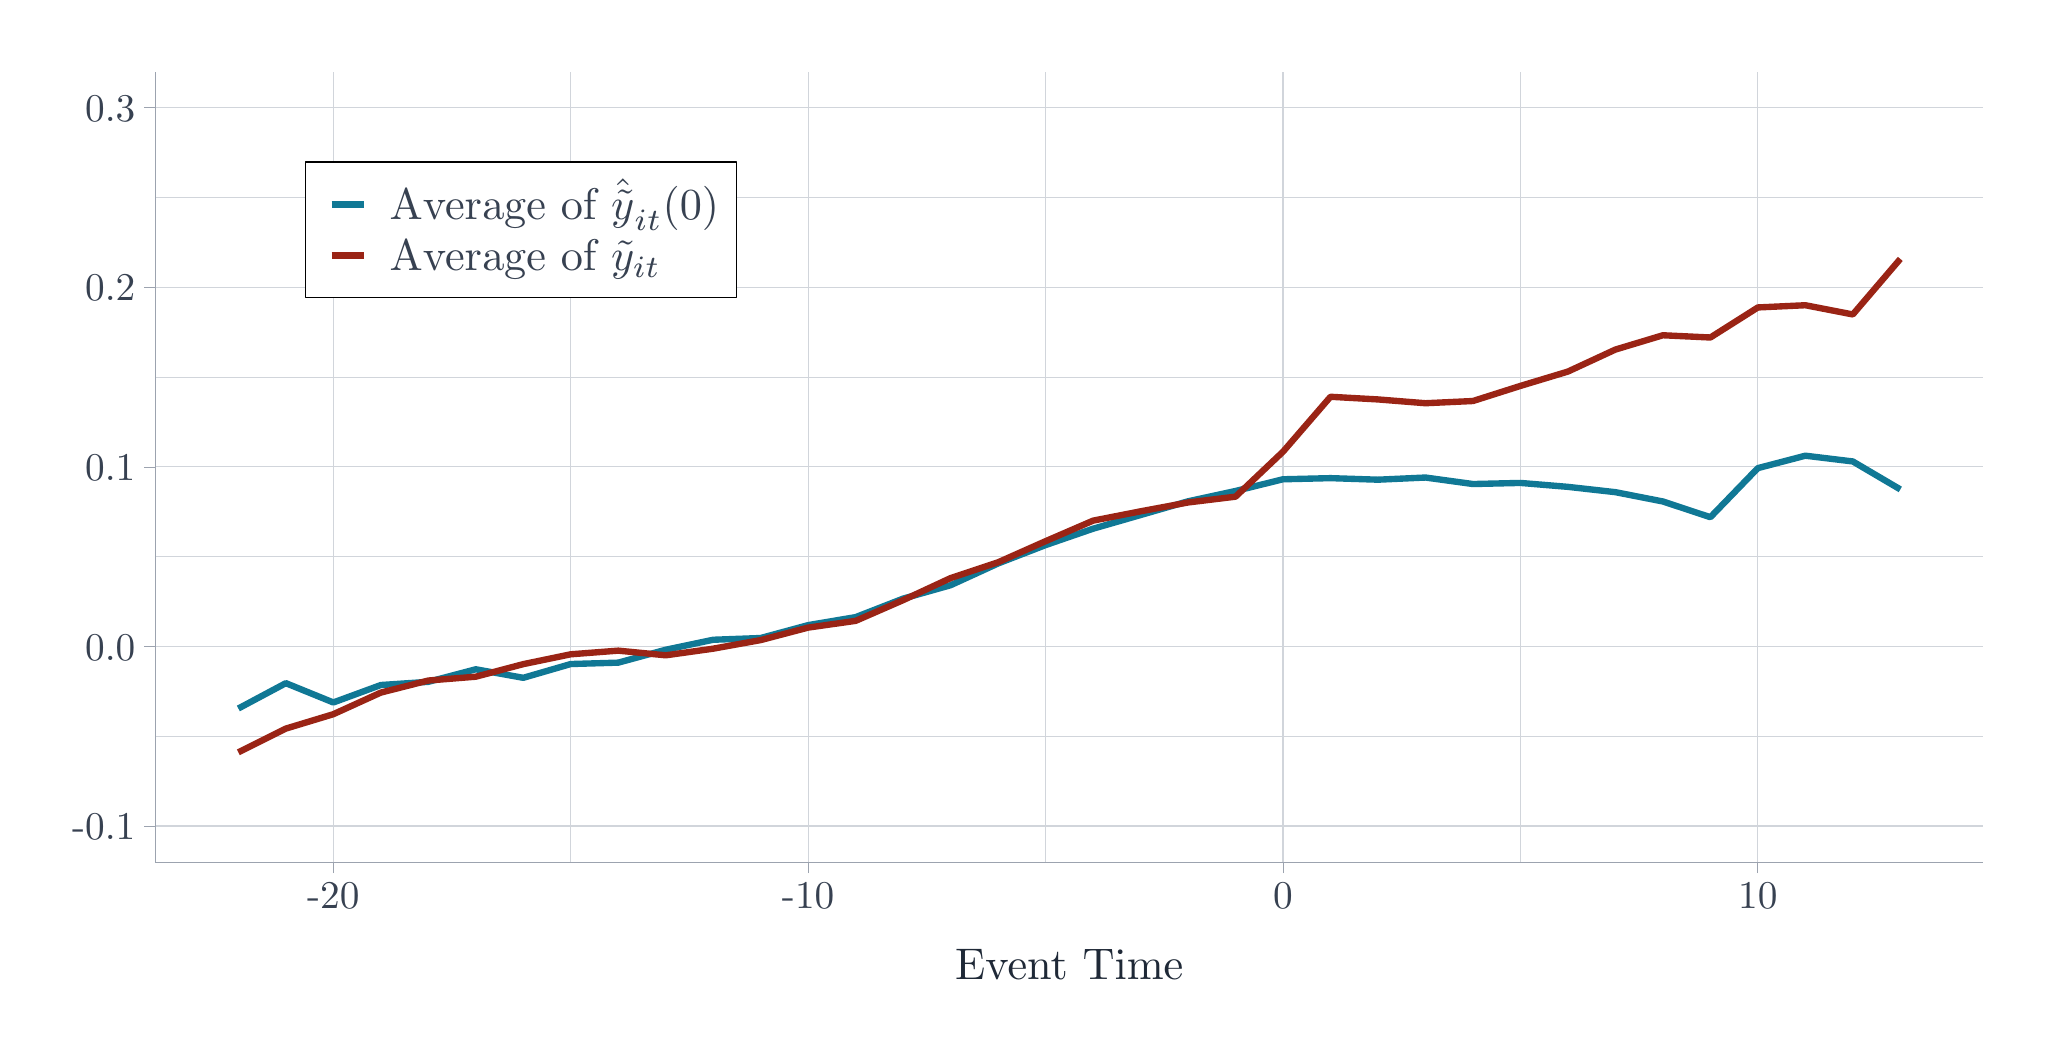
\begin{tikzpicture}[x=1pt,y=1pt]
\definecolor{fillColor}{RGB}{255,255,255}
\path[use as bounding box,fill=fillColor] (0,0) rectangle (722.70,361.35);
\begin{scope}
\path[clip] (  0.00,  0.00) rectangle (722.70,361.35);
\definecolor{drawColor}{RGB}{255,255,255}

\path[draw=drawColor,line width= 0.8pt,line join=round,line cap=round,fill=fillColor] (  0.00,  0.00) rectangle (722.70,361.35);
\end{scope}
\begin{scope}
\path[clip] ( 46.10, 59.89) rectangle (706.70,345.35);
\definecolor{drawColor}{RGB}{255,255,255}
\definecolor{fillColor}{RGB}{255,255,255}

\path[draw=drawColor,line width= 0.8pt,line join=round,line cap=round,fill=fillColor] ( 46.10, 59.89) rectangle (706.70,345.35);
\definecolor{drawColor}{RGB}{209,213,219}

\path[draw=drawColor,line width= 0.4pt,line join=round] ( 46.10,105.30) --
	(706.70,105.30);

\path[draw=drawColor,line width= 0.4pt,line join=round] ( 46.10,170.18) --
	(706.70,170.18);

\path[draw=drawColor,line width= 0.4pt,line join=round] ( 46.10,235.06) --
	(706.70,235.06);

\path[draw=drawColor,line width= 0.4pt,line join=round] ( 46.10,299.94) --
	(706.70,299.94);

\path[draw=drawColor,line width= 0.4pt,line join=round] (196.24, 59.89) --
	(196.24,345.35);

\path[draw=drawColor,line width= 0.4pt,line join=round] (367.82, 59.89) --
	(367.82,345.35);

\path[draw=drawColor,line width= 0.4pt,line join=round] (539.41, 59.89) --
	(539.41,345.35);

\path[draw=drawColor,line width= 0.4pt,line join=round] ( 46.10, 72.86) --
	(706.70, 72.86);

\path[draw=drawColor,line width= 0.4pt,line join=round] ( 46.10,137.74) --
	(706.70,137.74);

\path[draw=drawColor,line width= 0.4pt,line join=round] ( 46.10,202.62) --
	(706.70,202.62);

\path[draw=drawColor,line width= 0.4pt,line join=round] ( 46.10,267.50) --
	(706.70,267.50);

\path[draw=drawColor,line width= 0.4pt,line join=round] ( 46.10,332.37) --
	(706.70,332.37);

\path[draw=drawColor,line width= 0.4pt,line join=round] (110.45, 59.89) --
	(110.45,345.35);

\path[draw=drawColor,line width= 0.4pt,line join=round] (282.03, 59.89) --
	(282.03,345.35);

\path[draw=drawColor,line width= 0.4pt,line join=round] (453.61, 59.89) --
	(453.61,345.35);

\path[draw=drawColor,line width= 0.4pt,line join=round] (625.20, 59.89) --
	(625.20,345.35);
\definecolor{drawColor}{RGB}{16,120,149}

\path[draw=drawColor,line width= 2.3pt,line join=round] ( 76.13,115.33) --
	( 93.29,124.49) --
	(110.45,117.51) --
	(127.61,123.81) --
	(144.76,124.97) --
	(161.92,129.50) --
	(179.08,126.42) --
	(196.24,131.40) --
	(213.40,131.90) --
	(230.56,136.56) --
	(247.71,140.17) --
	(264.87,140.80) --
	(282.03,145.46) --
	(299.19,148.35) --
	(316.35,155.04) --
	(333.51,159.88) --
	(350.66,167.74) --
	(367.82,174.38) --
	(384.98,180.30) --
	(402.14,185.24) --
	(419.30,190.20) --
	(436.46,193.93) --
	(453.61,198.16) --
	(470.77,198.57) --
	(487.93,198.01) --
	(505.09,198.79) --
	(522.25,196.44) --
	(539.41,196.84) --
	(556.56,195.42) --
	(573.72,193.50) --
	(590.88,190.14) --
	(608.04,184.45) --
	(625.20,202.19) --
	(642.36,206.68) --
	(659.51,204.60) --
	(676.67,194.50);
\definecolor{drawColor}{RGB}{154,36,21}

\path[draw=drawColor,line width= 2.3pt,line join=round] ( 76.13, 99.51) --
	( 93.29,108.07) --
	(110.45,113.27) --
	(127.61,121.08) --
	(144.76,125.44) --
	(161.92,126.82) --
	(179.08,131.36) --
	(196.24,134.92) --
	(213.40,136.24) --
	(230.56,134.55) --
	(247.71,136.95) --
	(264.87,140.05) --
	(282.03,144.57) --
	(299.19,147.00) --
	(316.35,154.49) --
	(333.51,162.46) --
	(350.66,168.17) --
	(367.82,175.79) --
	(384.98,183.21) --
	(402.14,186.58) --
	(419.30,189.78) --
	(436.46,191.87) --
	(453.61,208.12) --
	(470.77,227.97) --
	(487.93,227.01) --
	(505.09,225.64) --
	(522.25,226.44) --
	(539.41,231.90) --
	(556.56,237.08) --
	(573.72,245.03) --
	(590.88,250.20) --
	(608.04,249.39) --
	(625.20,260.25) --
	(642.36,261.05) --
	(659.51,257.72) --
	(676.67,277.79);
\end{scope}
\begin{scope}
\path[clip] (  0.00,  0.00) rectangle (722.70,361.35);
\definecolor{drawColor}{RGB}{156,163,175}

\path[draw=drawColor,line width= 0.3pt,line join=round] ( 46.10, 59.89) --
	( 46.10,345.35);
\end{scope}
\begin{scope}
\path[clip] (  0.00,  0.00) rectangle (722.70,361.35);
\definecolor{drawColor}{RGB}{55,65,81}

\node[text=drawColor,anchor=base east,inner sep=0pt, outer sep=0pt, scale=  1.42] at ( 38.90, 67.97) {-0.1};

\node[text=drawColor,anchor=base east,inner sep=0pt, outer sep=0pt, scale=  1.42] at ( 38.90,132.84) {0.0};

\node[text=drawColor,anchor=base east,inner sep=0pt, outer sep=0pt, scale=  1.42] at ( 38.90,197.72) {0.1};

\node[text=drawColor,anchor=base east,inner sep=0pt, outer sep=0pt, scale=  1.42] at ( 38.90,262.60) {0.2};

\node[text=drawColor,anchor=base east,inner sep=0pt, outer sep=0pt, scale=  1.42] at ( 38.90,327.48) {0.3};
\end{scope}
\begin{scope}
\path[clip] (  0.00,  0.00) rectangle (722.70,361.35);
\definecolor{drawColor}{RGB}{156,163,175}

\path[draw=drawColor,line width= 0.3pt,line join=round] ( 42.10, 72.86) --
	( 46.10, 72.86);

\path[draw=drawColor,line width= 0.3pt,line join=round] ( 42.10,137.74) --
	( 46.10,137.74);

\path[draw=drawColor,line width= 0.3pt,line join=round] ( 42.10,202.62) --
	( 46.10,202.62);

\path[draw=drawColor,line width= 0.3pt,line join=round] ( 42.10,267.50) --
	( 46.10,267.50);

\path[draw=drawColor,line width= 0.3pt,line join=round] ( 42.10,332.37) --
	( 46.10,332.37);
\end{scope}
\begin{scope}
\path[clip] (  0.00,  0.00) rectangle (722.70,361.35);
\definecolor{drawColor}{RGB}{156,163,175}

\path[draw=drawColor,line width= 0.3pt,line join=round] ( 46.10, 59.89) --
	(706.70, 59.89);
\end{scope}
\begin{scope}
\path[clip] (  0.00,  0.00) rectangle (722.70,361.35);
\definecolor{drawColor}{RGB}{156,163,175}

\path[draw=drawColor,line width= 0.3pt,line join=round] (110.45, 55.89) --
	(110.45, 59.89);

\path[draw=drawColor,line width= 0.3pt,line join=round] (282.03, 55.89) --
	(282.03, 59.89);

\path[draw=drawColor,line width= 0.3pt,line join=round] (453.61, 55.89) --
	(453.61, 59.89);

\path[draw=drawColor,line width= 0.3pt,line join=round] (625.20, 55.89) --
	(625.20, 59.89);
\end{scope}
\begin{scope}
\path[clip] (  0.00,  0.00) rectangle (722.70,361.35);
\definecolor{drawColor}{RGB}{55,65,81}

\node[text=drawColor,anchor=base,inner sep=0pt, outer sep=0pt, scale=  1.42] at (110.45, 42.89) {-20};

\node[text=drawColor,anchor=base,inner sep=0pt, outer sep=0pt, scale=  1.42] at (282.03, 42.89) {-10};

\node[text=drawColor,anchor=base,inner sep=0pt, outer sep=0pt, scale=  1.42] at (453.61, 42.89) {0};

\node[text=drawColor,anchor=base,inner sep=0pt, outer sep=0pt, scale=  1.42] at (625.20, 42.89) {10};
\end{scope}
\begin{scope}
\path[clip] (  0.00,  0.00) rectangle (722.70,361.35);
\definecolor{drawColor}{RGB}{31,41,55}

\node[text=drawColor,anchor=base,inner sep=0pt, outer sep=0pt, scale=  1.60] at (376.40, 17.56) {Event Time};
\end{scope}
\begin{scope}
\path[clip] (  0.00,  0.00) rectangle (722.70,361.35);
\definecolor{drawColor}{RGB}{0,0,0}
\definecolor{fillColor}{RGB}{255,255,255}

\path[draw=drawColor,line width= 0.6pt,line join=round,line cap=round,fill=fillColor] (100.36,263.80) rectangle (256.09,312.71);
\end{scope}
\begin{scope}
\path[clip] (  0.00,  0.00) rectangle (722.70,361.35);
\definecolor{drawColor}{RGB}{255,255,255}
\definecolor{fillColor}{RGB}{255,255,255}

\path[draw=drawColor,line width= 0.8pt,line join=round,line cap=round,fill=fillColor] (108.36,290.26) rectangle (122.81,304.71);
\end{scope}
\begin{scope}
\path[clip] (  0.00,  0.00) rectangle (722.70,361.35);
\definecolor{drawColor}{RGB}{16,120,149}

\path[draw=drawColor,line width= 2.3pt,line join=round] (109.81,297.48) -- (121.37,297.48);
\end{scope}
\begin{scope}
\path[clip] (  0.00,  0.00) rectangle (722.70,361.35);
\definecolor{drawColor}{RGB}{255,255,255}
\definecolor{fillColor}{RGB}{255,255,255}

\path[draw=drawColor,line width= 0.8pt,line join=round,line cap=round,fill=fillColor] (108.36,271.80) rectangle (122.81,286.26);
\end{scope}
\begin{scope}
\path[clip] (  0.00,  0.00) rectangle (722.70,361.35);
\definecolor{drawColor}{RGB}{154,36,21}

\path[draw=drawColor,line width= 2.3pt,line join=round] (109.81,279.03) -- (121.37,279.03);
\end{scope}
\begin{scope}
\path[clip] (  0.00,  0.00) rectangle (722.70,361.35);
\definecolor{drawColor}{RGB}{55,65,81}

\node[text=drawColor,anchor=base west,inner sep=0pt, outer sep=0pt, scale=  1.60] at (130.81,291.97) {Average of $\hat{\tilde{y}}_{it}(0)$};
\end{scope}
\begin{scope}
\path[clip] (  0.00,  0.00) rectangle (722.70,361.35);
\definecolor{drawColor}{RGB}{55,65,81}

\node[text=drawColor,anchor=base west,inner sep=0pt, outer sep=0pt, scale=  1.60] at (130.81,273.52) {Average of $\tilde{y}_{it}$};
\end{scope}
\end{tikzpicture}
